
\documentclass[12pt]{article}

%
%Margin - 1 inch on all sides
%
\usepackage[letterpaper]{geometry}
\usepackage{times}
\geometry{top=1.0in, bottom=1.0in, left=1.0in, right=1.0in}

%
%Doublespacing
%
\usepackage{setspace}
\doublespacing

% justify
\usepackage{ragged2e}

%
%Rotating tables (e.g. sideways when too long)
%
\usepackage{rotating}

%
% Indent the first paragraph after section title
%
\usepackage{indentfirst}

% use roman numerals for section and subsection
\renewcommand{\thesection}{\Roman{section}} 
\renewcommand{\thesubsection}{\thesection.\Roman{subsection}}

%
%allow counting superscript
%
\usepackage[super]{nth}

% set size of section title
\usepackage{titlesec}
\titleformat*{\section}{\normalfont\bfseries}
\titleformat*{\subsection}{\normalfont\bfseries}

%
%Fancy-header package to modify header/page numbering (insert last name)
%
\usepackage{fancyhdr}
\pagestyle{fancy}
\lhead{} 
\chead{} 
\rhead{He \thepage} 
\lfoot{} 
\cfoot{} 
\rfoot{} 
\renewcommand{\headrulewidth}{0pt} 
\renewcommand{\footrulewidth}{0pt} 
%To make sure we actually have header 0.5in away from top edge
%12pt is one-sixth of an inch. Subtract this from 0.5in to get headsep value
\setlength\headsep{0.333in}


%
%Works cited environment
%(to start, use \begin{workscited...}, each entry preceded by \bibent)
% - from Ryan Alcock's MLA style file
%
\newcommand{\bibent}{\noindent \hangindent 40pt}
\newenvironment{workscited}{\newpage \begin{center} Works Cited \end{center}}{\newpage }


%
%Begin document
%
\begin{document}
\begin{flushleft}

%%%%First page name, class, etc
Ethan He \\
Professor Miller \\
UWP 001 \\
September 11 2020 \\

% title
\begin{center}
    \textbf{Gaining Voice: Transformations of the Undocumented Youth Movement in CIJYA}
\end{center}

%%%%Changes paragraph indentation to 0.5in
\setlength{\parindent}{0.5in}
%%%%Begin body of paper here

% !! explain the quote and source, what are yuo trying to argue? bridging 

\section*{Introduction}

In the past decades, more undocumented youth have come of the shadows to struggle against the criminalization and discrimination they encountered and fight for their rights in community, society, and the United States. 
Among the surging youth-led alliances, California Immigrant Youth Justice Alliance (CIYJA) is one of the most influential organizations that focus on placing undocumented youth in advocacy and policy delegations. 
By strategically employing the empowering practice of storytelling, the CIYJA launches transformational movement that goes beyond narrowly defined legalization and manages to empower the community members with agency.
% 1). that can apply to any organization; 2). what does it means fir diverse communities.
% rely on __ kinds of storytelling to ___ . 
% how do they make changes?

Narrative has been widely discussed as a powerful tool to (re)construct reality and empower the marginalized groups in society. 
Jerome Bruner, the co-founder of Center for Cognitive Studies at Harvard, has argued that one of the important ways people understand their world is through storytelling, in which people express their wants, needs, and goals (1). 
In the similar vein, Davis points out that ``social movements are dominated by stories and storytelling, and narratives goes to the heart of the very cultural and ideational processes, including public discourse, movement culture, … and collective identity (4). 
Riessman also stresses the ability of narratives to ``do political work'' (8) in constructing norms, identities and ideologies. 
Although playing a critical role in social movements, storytelling and its transformational power has been relatively neglected in the research on undocumented youth community. 
In an attempt to organize diverse communities, the CIYJA uses storytelling to connect different fights against the anti-migration hegemony. 
This paper examines how the CIYJA's members tell their stories in different forms and how these narratives are employed strategically to achieve diverging goals, including giving voice to community members, expanding the Dreamer narrative, and mobilizing undocumented youth as well as the public. 
Three stories from different platforms of CIYJA are select and analyzed in the following sections to showcase their efficiency to serve the common goals of the organization. 


\section*{Storytelling (re)constructs and negotiates identity}

Storytelling is a powerful way to voice experiences and share and transform individual and collective identities (De Fina 1). 
In this way, storytelling helps the community members gain their voice. The story selected in this section is from Mariela Mendez, the Cultivator of Change with CIYJA, in an article under the title of ``\textit{Our Voices Will Not be Drowned}'' on CIYJA's website. In her story, Mariela shares her experience of coming out shadows painstakingly yet bravely: 

\begin{quotation}
    \noindent
    My family's time here has been a story of shadows. $\ldots$ [T]hese shadows have silenced me.
    For some odd reason, I felt that it was necessary to remain quiet and unseen from protests that involved controversy. 
    I didn't want to implicate or worry about my family.
    I still recall living in the shadows with fear, and uncertainty in my future.
    Despite knowing that the rhetoric and terms used to identify the undocumented community led to the unethical and inhumane treatment I experienced, I was okay with living in the shadows.
\end{quotation} % source-checked

\noindent
As most undocumented youth, Mariela initially accepted the social identity assigned to her and her community, and ``was OK living in the shadows'' until an incident at the TRUTH Forum in August 2018, where she witnessed paid agitator yelling out racist and homophobic slurs at them, a group of local undocumented youth helping with organizing the forum.
By recalling and reflecting the experience, Mariela gained determination and bravery to rise up from the shadows regardless of her legal status.
Suganami, the profess of Department of International Politics at Aberystwyth University, suggests that narratives are essential to community building and (re)constructing a common identity (366).
In this case, Mariela not only (re)constructs and negotiates her collective identity within the community, but more importantly, she obtains subjectivity, a sense of agency, to reject and resist the assigned identity and make assertive claims, as she narrates at the end of her story:

\begin{quotation}
    \noindent
    I know that in order to start living out of shadows, I must not be afraid to stand up for what I believe in, and I must learn to be fearless.
    It is of vital importance for all who have immigrated to the U.S. with or without a current legal status to come out of the shadows in order to raise awareness and publicly advocate for themselves.
\end{quotation} % source-checked

\noindent
This story shared on the CIYJA's website with most of its audiences as undocumented youth and supporters works effectively to gain voice to used-to-be silent groups. 
By giving themselves new, positive identities, undocumented youth are empowered to challenge anti-immigrant rhetoric and advocate for themselves.

\section*{Storytelling builds diverse communities}

Storytelling, with it emotional, cultural mechanism, can be used as a powerful tool to build more diverse communities (Swerts 347). % source-checked
One story shared on the CIYJA's website, which challenges the narrative of ``Dreamer'', serves such a goal as promoting a more inclusive, diverse community by directly opposing the criminalization of undocumented youth.
Since the DREAM Act passed in 2019 after years of debate, the term ``Dreamer'' has been increasingly used by researchers and community members as a collective identity of undocumented youth. However, despite its function in generating and maintaining movement and promoting collective action (Fiorito), this term has been rejected by more undocumented youth and movement organizers for its labeling implication and exclusive effect. For example, Edna, the CIYJA organizer suggests, ``[The term] was kinda helpful, but at the same time I think we really thought about the consequences of how it would create the two categories: `good immigrant' versus `bad immigrant''' (Schwiertz 615). Edna' statement point out the necessity of going beyond the term. Similarly, under the title of ``\textit{Take It from the Central Valley: You're Using the Wrong Narrative}'', Brisa Cruz, the Central California Regional Organizer with CIYJA, shares her disappointment when reading such a well-meaning article as ``\textit{Want to Send Dreamers back to Mexico? If you met one, you'd probably change your mind}'' on the news website of The Fresno Bee: 

\begin{quotation}
    \noindent
    The story only associates the current immigration climate with the so called ``Dreamers,'' a label that I strongly dislike and have never identified with.
    I am a DACA recipient myself and understand the privilege I have; however, a social security number and an Employment Authorization Card doesn't mean I have stopped fighting for the human dignity and liberation of my community--the same community that continues to be criminalized and tokenized by those in power.
\end{quotation} % source-checked

\noindent
In her narrative, Brisa showed her strong emotions about being thrust upon the rhetoric of ``Dreamer''. Her advocate in the later article to find ``creative, inclusive alternatives that involves everyone in our diverse community'', demonstrate how storytelling, as relates to emotions, can raise self- and other's awareness of destructing the narrowly defined narrative. In an attempt to organize diverse communities, the CIYJA also uses storytelling to connect different fights against the anti-migration hegemony. In a video clip posted by Daniel Alvarenga and retweeted by the CIYJA, several Cameroonian immigrants detained at Pine Prairie ICE shared their stories of being caught and locked up in solitary confinement. In the campaign of ``Free Them All'', Ciyia Valeria, on her Instagram post, read a letter from someone detained at Mesa Verde Detention Facility, telling their unknown stories in the facility. These stories display the diversity of the undocumented community and build a more inclusive movement. 

\section*{Storytelling makes claims}

Besides displaying their emotions, concerns as the subject of brutal policing, incarceration and deportation, all these self- and other-told stories also serve as ``significant part of extra-movement communication with the media, public and politicians'' (Swerts 355). When being purposely used in different contexts and told to different audience, the stories provide the moral grounds to gain public support. In the petition of ``Help Erika Return to Her Family'' made to Congress members by the CIYJA, the petition organizers told the story of how Erica and her family struggled for her legal citizenship. Having lived in the Central Valley since 1999, Erica was rejected in a visa application in 2014 due to a previous unauthorized re-entry into the U.S when she was a minor back in 2006. The story was posted on the CIYJA's website, the social media, and in the public letters to the congress members. By appealing to logos and pathos, this type of storytelling provides politicians with the moral and emotional resources necessary to legitimate their support, as Swerts (356) in his paper states. By telling stories to urge Congress members to help Erika obtain discretion in her case, the CIYJA makes the appeal that ``We need more politicians to take a public stance against the rogue undermining of the current administration, for the safety of all targeted communities''. In this way of sharing personal stories, the organization mobilizes the public by building intimacy with those who might be disconnected with their activities. 

\section*{Storytelling with images to appeal to pathos}

Besides narrated stories, CIYJA also employs images to convey the messages of promoting prison abolition and to appeal to the public's support. One piece of illustrated news on the CIYJA's website under the title ``\#FREETHEMALL: Incarceration is a Health Hazard, We Merely Got a Glimpse of It'' demonstrate clearly the power of virtual texts in appealing to pathos and conveying messages (see Figure1). 

\newpage
\begin{figure}[h]
    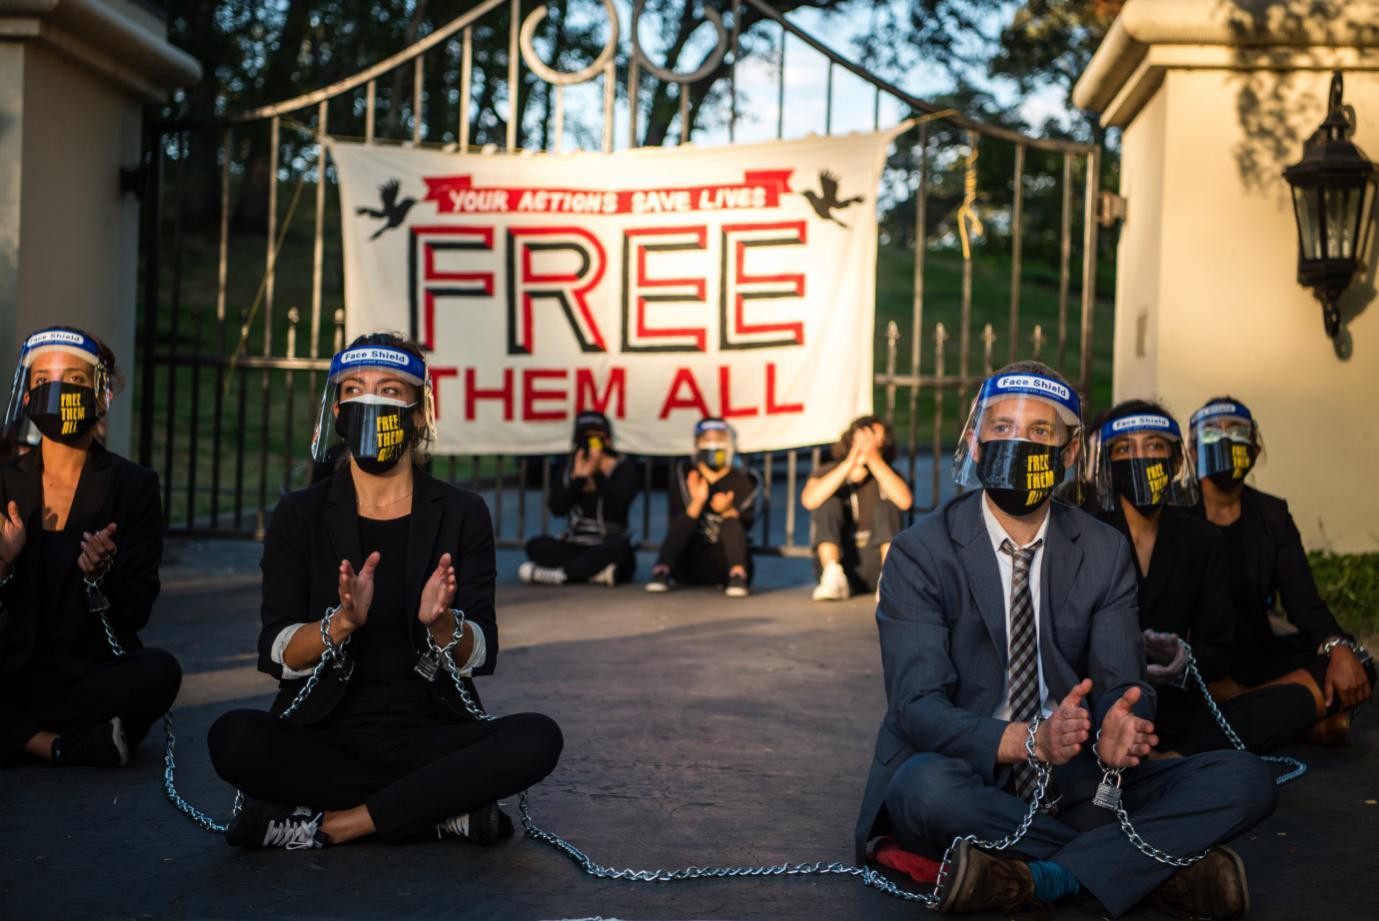
\includegraphics[width=0.95\textwidth]{./Figure1.png}
    \caption{``FREETHEMALL: Incarceration is a Health Hazard, We Merely Got a Glimpse of It''. CIYJA. https://ciyja.org/freethemall14chronicle/}
    \label{Figure 1}
\end{figure}

In the foreground the image, five persons of different colors with their facial masks and goggles are sitting in a half-circle, with their wrists chained to each other. Three of them seem to be clapping. The background of the image is an iron gate covered with a huge sign that prints ``FREE THEM ALL'' in striking red and a flying bird on each top corner. Three other persons with facial masks and goggles as well (except one) are sitting under the sign, leaning on the gate, and the one without masks covers his face with his hands. The same face shields and face masks along with the chains unify the protesters. 

According to the website, it was a statement made by 14 immigration attorneys who are actually protesting, undocumented organizers and supports who locked themselves to each other and to the gate of California Governor's mansion, demanding he used his authority to protect the lives of those incarcerated in California state prisons and detention facilities. The intended purpose of the image is very clear: to explain the goal of the statement to the community members and other potential audiences by appealing to pathos and ethos. The chains that lock the activists together effectively evoke emotions from viewers, showing them the determination and strategies of the activities to change the representation of political power in the state. Since they are chained together, they are making it harder for them to be removed by police. By highlighting one of the male activists in suits and tie, the image establishes ethos of this statement by implying his identity: an attorney who supports undocumented community. The intended audience of the image are the CIYJA users, including its organizers, members, and other supporters who have the chance to browse its website. The picture is also posted on the organization's social media like Tweeter, Facebook, and Instagram, so it aims to reach more audience who are interested in the organization's missions and campaigns. 

As one phrase goes, ``a picture is worth a thousand words''. It is true in this case, where the image conveys more messages with its denotation as well as connotation. The chains that lock the activists to each other and to the gate connotate not merely restraint, but power and support. By locking themselves together in front of the iron gate, the activists are imitating those who are locked up in prisons and other detention facilities. These visible chains and gate are reminding viewers the bars behind which undocumented individuals are incarcerated as well as invisible restraints and threats of those incarcerated people encounter. On the other hand, the chains connotate the organizers' collective power and solidarity as well. By locking themselves together, the activists show that they are in an unbroken community with the common aim to fight against authoritative hegemony represented by the mansion's gate. 

All the activists in the picture except one who covers his face with his hands wear three layers of protection: a white surgical mask inside, a black mask which writes, ``Free Them All!'' in striking yellow, and goggles. These gears denote protection from the current virus. While people outside prisons have the choice to wear masks, goggles, and keep social distancing, do those incarcerated have the same rights? The masks and goggles also connotate protection from the law enforcement and government. It reminds me of a slogan I saw on a prison abolition website: ``Prisons are Pandemics''. It is true that in current situation, prisons are even worse than the pandemic, which hopefully will exist around us only for a short period. However, prisons and incarceration are something more horrible and eradicable. They threaten and kill all those powerless, marginalized individuals, and communities. 

\section*{Conclusion}

Storytelling is powerful assets for marginalized communities and individuals. By giving their voices, reconstructing their identities and subjectivity, and justifying their claims, these stories connect not only the community members but also the human history. As Emanuel, a member and supporter of CIYJA, claims in the ``Coming out of the Shadows'' protest, ``Undocumented immigrants are the backbone of the entire southwest region of the United States, and we are not going anywhere.'' (\textit{CIYJA})

%%%%Works cited
\begin{workscited}

\bibent
Bruner, Jerome. ``The Narrative Construction of Reality.'' \textit{Critical Inquiry}. 18.1 (1991): 1-21.

\bibent
Cruz, Brisa. ``Take It from the Central Valley: You're Using the Wrong Narrative''. \textit{CIYJA}. https://ciyja.org/take-it-from-the-central-valley/

\bibent
Davis, Joseph E. \textit{Stories of Change: Narrative and Social Movements}. State University of New York Press, 2002.

\bibent
De Fina, Anna. \textit{Identity in Narrative: A study of Immigrant Discourse}. Vol. 3. John Benjamins Publishing, 2003.

\bibent
Mendez, Mariela. ``Our Voices Will Not Be Drowned''. \textit{CIYJA}. https://ciyja.org/our-voices-will-not-be-drowned/

\bibent
Riessman, Catherine Kohler. \textit{Narrative Methods for the Human Sciences}. Sage Publications, 2007.

\bibent
Schwiertz, Helge. ``Transformations of the Undocumented youth movement and radical egalitarian citizenship.'' \textit{Citizenship Studies}, vol. 20, no. 5, 2016, pp.610-628.

\bibent
Servin, John. ``Press Release: Kern Country `Coming out of the Shadows'''. \textit{CIYJA}. https://ciyja.org/kern-county-coming-out-of-the-shadows-march-23/

\bibent
Suganami, Hidemi. "Agents, structures, narratives." European Journal of International Relations 5.3 (1999): 365-386.

\bibent
Swerts, Thomas. ``Gaining a voice: Storytelling and undocumented youth activism in Chicago.'' Mobilization: An International Quarterly, vol. 20, no. 3, 2015, pp. 345-360.

\bibent
``Take Action: Help Erika Return To Her Family''. \textit{CIYJA}. https://ciyja.org/petitions/
\end{workscited}

\end{flushleft}
\end{document}
